\documentclass{article}

\usepackage{graphicx}
\usepackage{tikz}
\usepackage{tikzsymbols}
\usetikzlibrary{calc,patterns,shapes.geometric}
\pagestyle{empty}
\usepackage[margin=0pt]{geometry}
\geometry{papersize={14in,12in}}

\def\centerarc[#1](#2)(#3:#4:#5){\draw[#1] ($(#2)+({#5*cos(#3)},{#5*sin(#3)})$) arc (#3:#4:#5);}

\begin{document}
	\begin{figure}
		\centering
		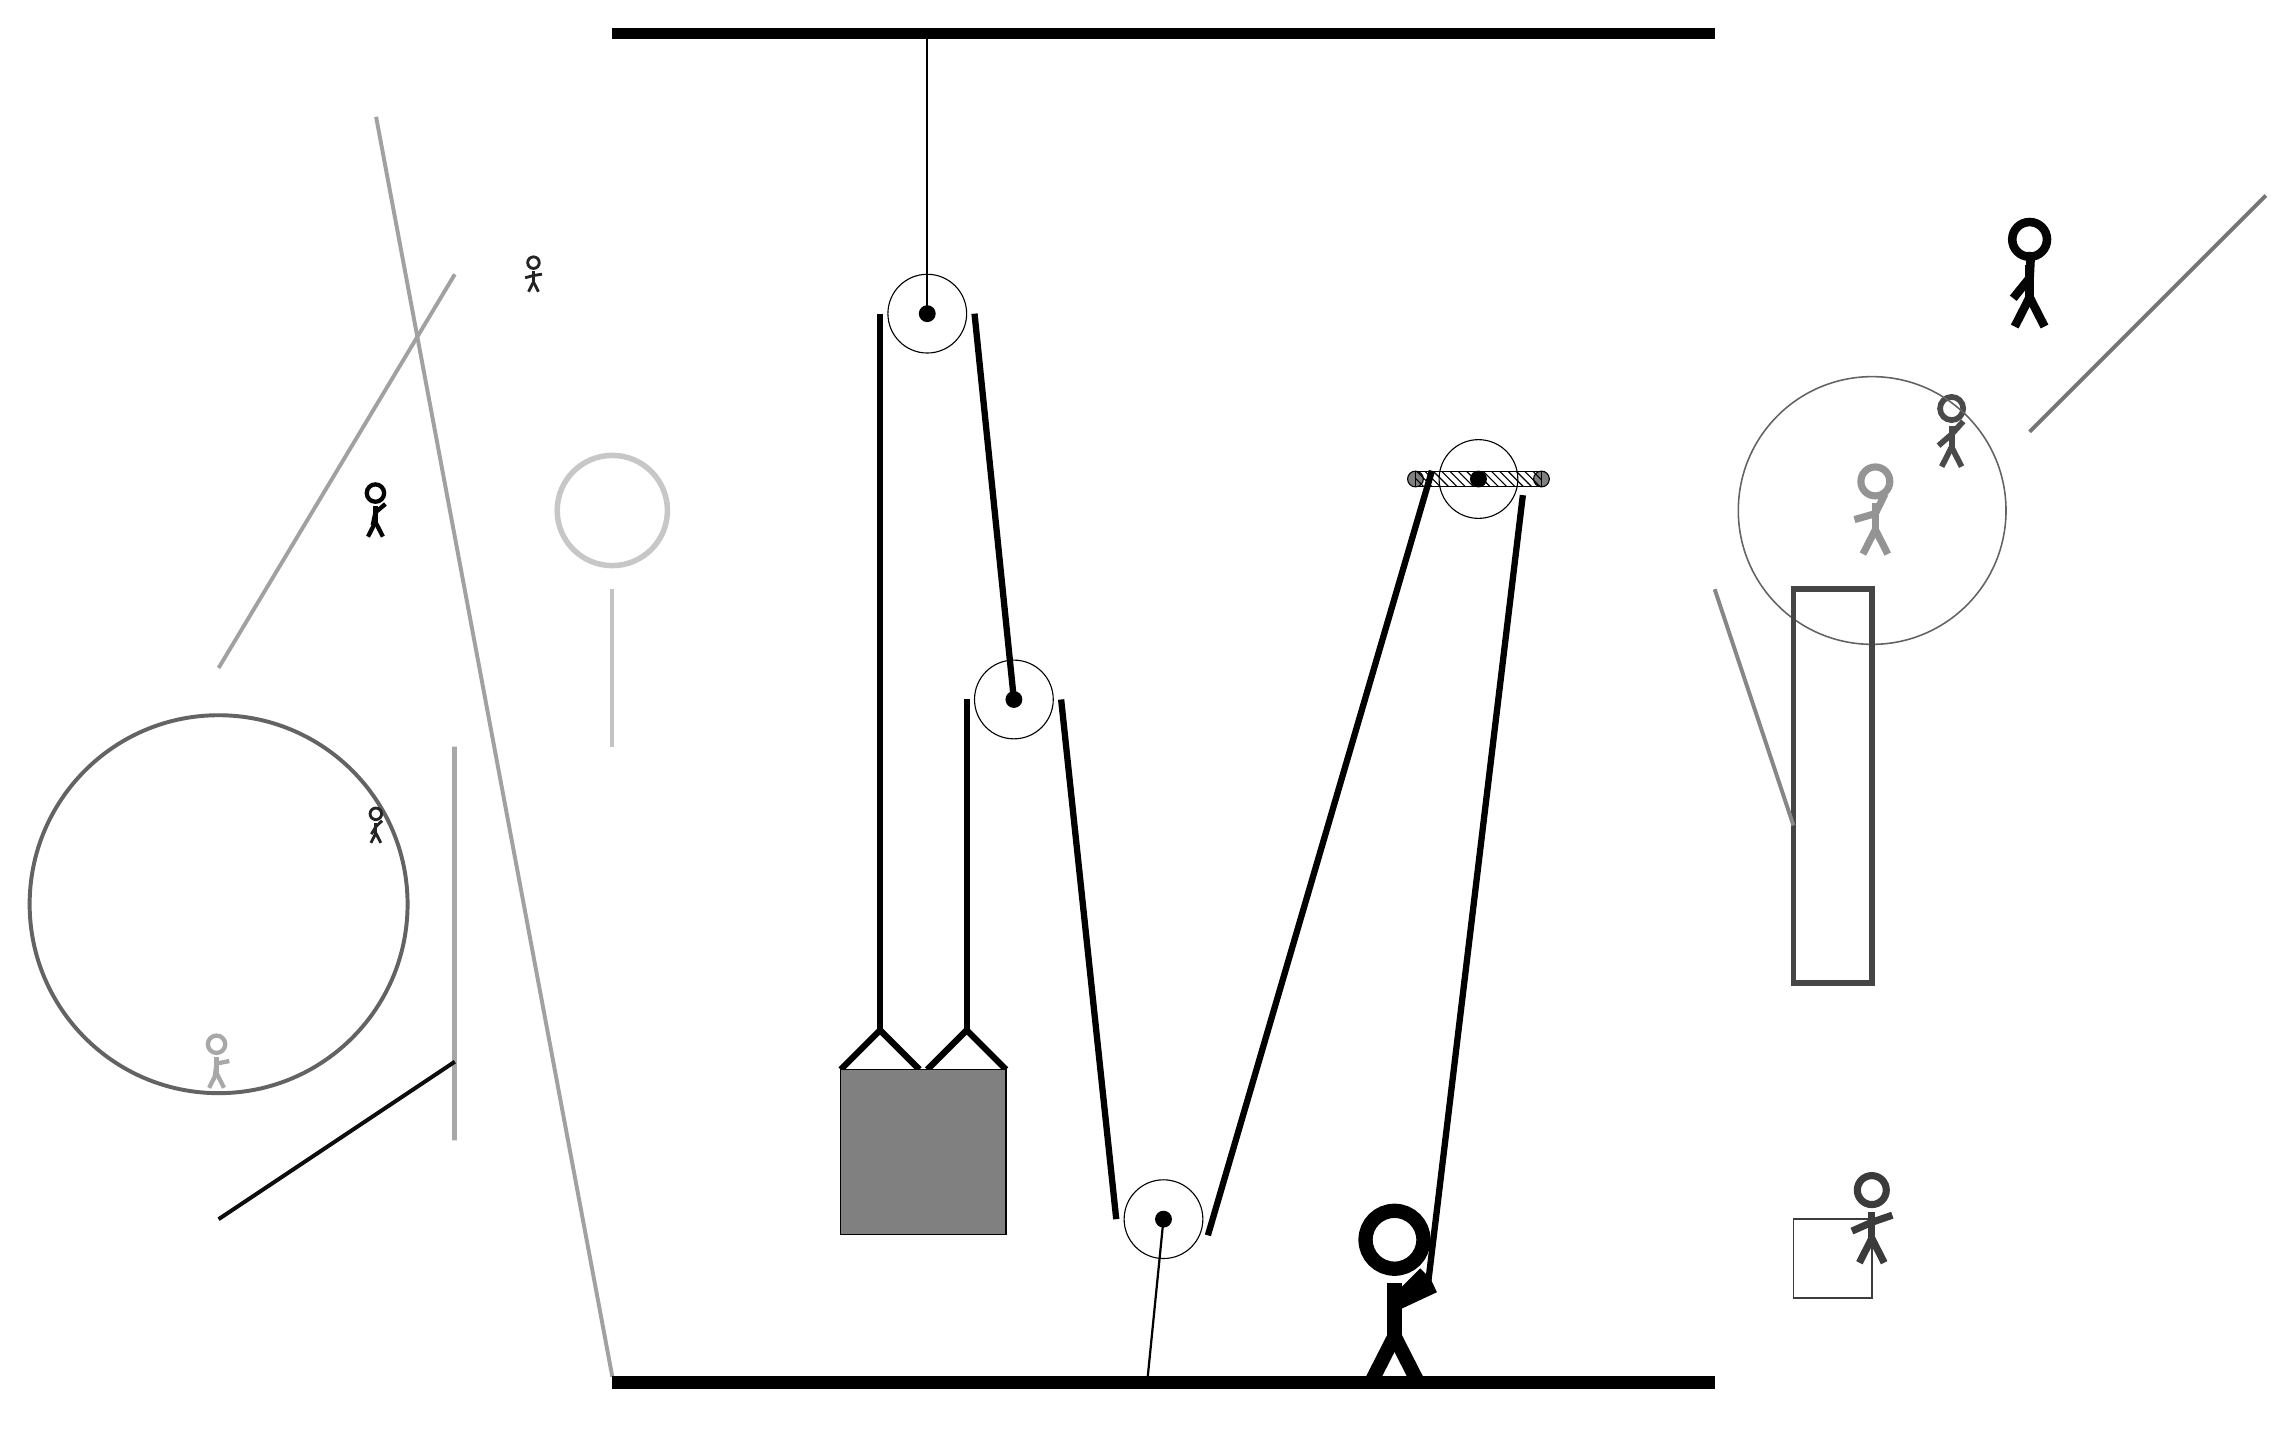
\begin{tikzpicture}
			%%%%% START %%%%%
			
			\draw[fill=black] (-2, 14) rectangle (12, 14.125);
			
			\draw (2, 10.5) circle (0.5);
			\draw[fill=black] (2, 10.5) circle (0.1);
			\draw[thick] (2, 10.5) -- (2, 14);
			
			\draw[line width=0.5mm, color=black!37](-5, 13) -- (-2, -3);
			
			\node[line width=0.4mm, color=black!77] at (14, -1) {\Strichmaxerl[5][24][19]};
			\draw[line width=0.5mm, color=black!23](-2, 7) -- (-2, 5);
			\draw[line width=0.5mm, color=black!54](16, 9) -- (19, 12);
			\draw[line width=0.6mm, color=black!34] (-4, 5) rectangle (-4, 0);
			\draw[line width=0.5mm, color=black!37](-7, 6) -- (-4, 11);
			\draw [line width=0.5mm, color=black!61](-7, 3) circle (2.4);
			
			\node[line width=0.2mm, color=black!98] at (16, 11) {\Strichmaxerl[6][51][87]};
			\draw[line width=0.2mm, color=black!76] (13, -2) rectangle (14, -1);
			
			\draw [line width=0.7mm, color=black!22](-2, 8) circle (0.7);
			\node[line width=0.2mm, color=black!71] at (15, 9) {\Strichmaxerl[4][41][48]};
			\draw [line width=0.2mm, color=black!61](14, 8) circle (1.7);
			\node[line width=0.7mm, color=black!86] at (-3, 11) {\Strichmaxerl[2][15][9]};
			
			\node[line width=0.4mm, color=black!42] at (14, 8) {\Strichmaxerl[5][16][64]};
			\draw[line width=0.5mm, color=black!95](-4, 1) -- (-7, -1);
			\draw[line width=0.7mm, color=black!73] (14, 2) rectangle (13, 7);
			
			\node[line width=0.5mm, color=black!34] at (-7, 1) {\Strichmaxerl[3][82][11]};
			\node[line width=0.2mm, color=black!98] at (-5, 8) {\Strichmaxerl[3][78][40]};
			\draw[line width=0.5mm, color=black!47](13, 4) -- (12, 7);
			\node[line width=0.3mm, color=black!86] at (-5, 4) {\Strichmaxerl[2][59][44]};
			
			\draw (3.1, 5.6) circle (0.5);
			\draw[fill=black] (3.1, 5.6) circle (0.1);
			
			\draw (5, -1) circle (0.5);
			\draw[fill=black] (5, -1) circle (0.1);
			\draw[thick] (5, -1) -- (4.8, -3);
			
			\draw (9, 8.4) circle (0.5);
			\draw[fill=black] (9, 8.4) circle (0.1);
			\draw[fill=black!50] (8.2, 8.4) circle (0.1);
			\draw[fill=black!50] (9.8, 8.4) circle (0.1);
			\draw[pattern=north west lines, pattern color=black] (8.2, 8.5) rectangle (9.8, 8.3);
			
			\draw[line width = 0.8mm]  (0.9, 0.9) -- (1.4, 1.4) -- (1.9, 0.9);
			\draw[line width = 0.8mm]  (2.0, 0.9) -- (2.5, 1.4) -- (3.0, 0.9);
			\draw[fill=black!50] (0.9, 0.9) rectangle (3.0, -1.2);
			
			\draw[line width = 0.8mm] (1.4, 10.5) -- (1.4, 1.4);
			\centerarc[line width = 0.8mm](2, 10.5)(0:180:0.6);
			\draw[line width = 0.8mm] (2.6, 10.5) -- (3.1, 5.6);
			\draw[line width = 0.8mm] (2.5, 5.6) -- (2.5, 1.4);
			\centerarc[line width = 0.8mm](3.1, 5.6)(0:180:0.6);
			\draw[line width = 0.8mm] (3.7, 5.6) -- (4.4, -1);
			\centerarc[line width = 0.8mm](5, -1)(180:340:0.6);
			\draw[line width=0.8mm](5.5638, -1.2052) -- (8.4091, 8.5042);
			\centerarc[line width = 0.8mm](9, 8.4)(-20:170:0.6);
			\draw[line width=0.8mm](9.5638, 8.1948) --  (8.35, -1.9);
			
			\node at (8, -2) {\Strichmaxerl[10][225][25]};
			
			\draw[fill=black] (-2, -3) rectangle (12, -3.15);
			
			%%%%% END %%%%%
		\end{tikzpicture}
	\end{figure}	
\end{document}